
\section{Low Speed Wind Tunnel}

The Old Dominion University low 
speed wind tunnel (LSWT) was outfitted with a bi-wing axial vortex generator. 
The tunnel has a large test section measuring 2.134$m$ wide by 2.438$m$ 
tall and a smaller, higher speed test section measuring 1.219$m$ wide by 
0.911$m$ tall (3 x 4 feet). The 
wind tunnel air is propelled with a frequency controlled 125 horsepower motor. 
Flow velocity was manipulated directly by manually controlling
voltage supplied to the controller. 
The small test section, used in the present experimental investigation, has a 
total length of 2.438$m$, and the vertically mounted vortex generator 
spanned the 0.911$m$ height of the test section and was 
mounted 0.610$m$ from the end of the flow contraction section, leaving 1.829$m$ 
downstream for the axial 
vortex to develop. The high speed test section has a functional free stream 
velocity range between 12 and 55  $m/s$ or between 35 and 120 $mph$.

\begin{figure}[H]
\centering
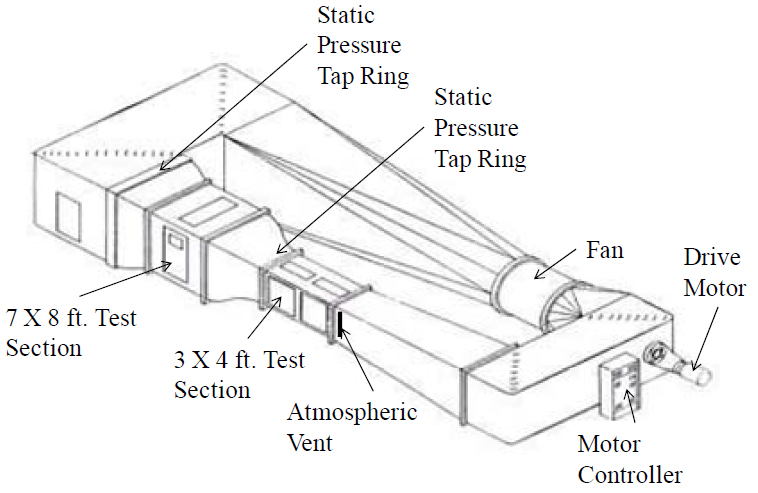
\includegraphics[width=5in]{figs/setup/odulswt_diagram}
\caption{ODU Low speed wind tunnel.}
\label{fig:odulswt}
\end{figure}

The entire interior of the test section was vacant and unobstructed beyond the 
vortex generator. 
No internal traverse systems or structures 
were present during PIV data acquisition unless otherwise indicated. Tunnel 
velocity was determined by direct measurement of dynamic pressure ($q$), which 
is monitored and controlled by the tunnel control PC. A functional schematic of 
the LSWT PC-based tunnel control system is shown in Figure 
\ref{fig:control_diagram}

\begin{figure}[H]
\centering
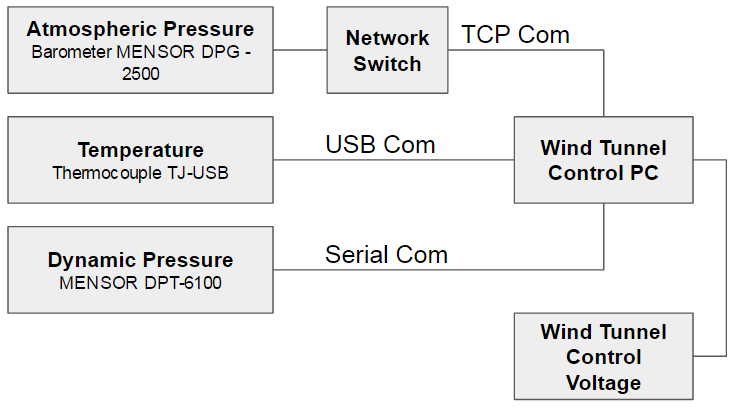
\includegraphics[width=5in]{figs/setup/odulswt_control}
\caption{Schematic diagram of systems under wind tunnel PC control.}
\label{fig:control_diagram}
\end{figure}


